% Created by tikzDevice version 0.12.3.1 on 2022-09-02 14:29:32
% !TEX encoding = UTF-8 Unicode
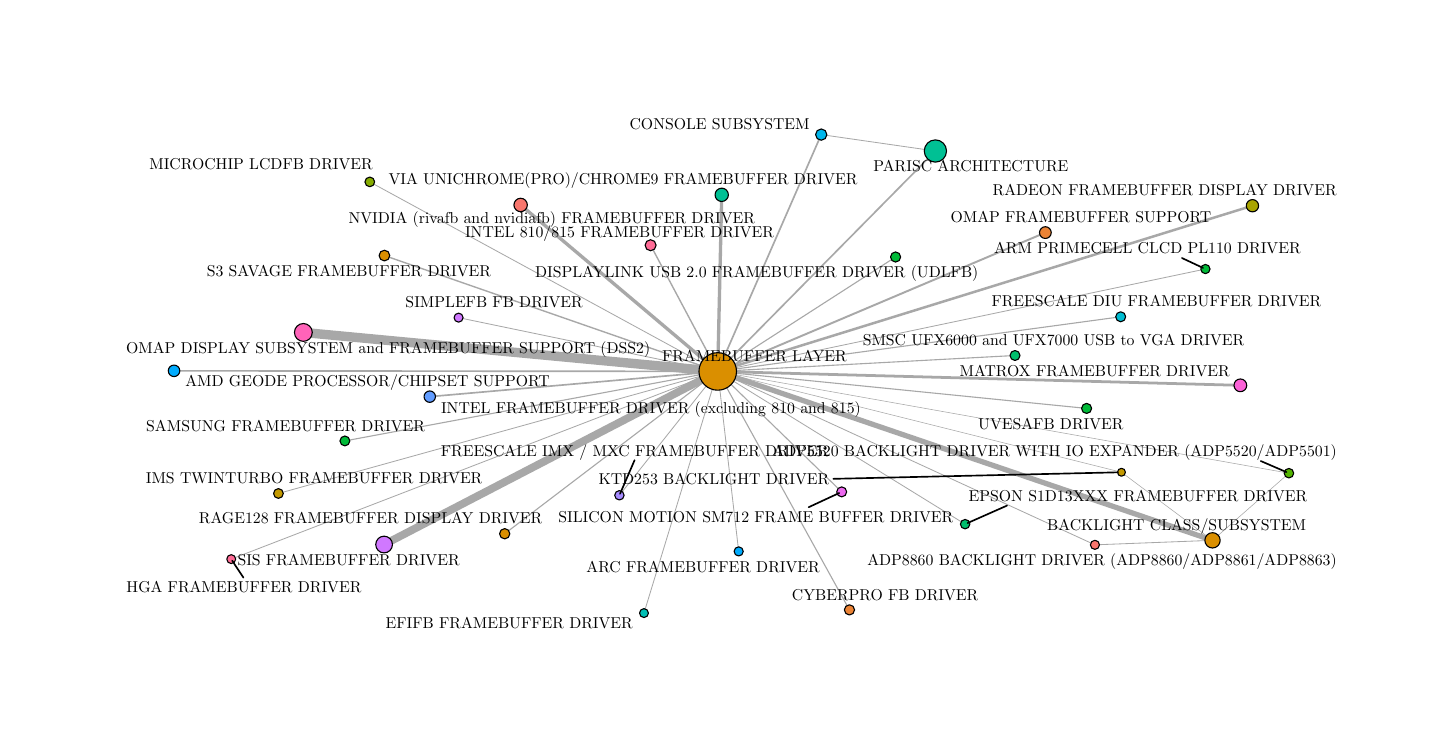
\begin{tikzpicture}[x=1pt,y=1pt]
\definecolor{fillColor}{RGB}{255,255,255}
\path[use as bounding box,fill=fillColor,fill opacity=0.00] (0,0) rectangle (505.89,252.94);
\begin{scope}
\path[clip] (  0.00,  0.00) rectangle (505.89,252.94);
\definecolor{fillColor}{RGB}{255,255,255}

\path[fill=fillColor] (  0.00,  0.00) rectangle (505.89,252.94);
\end{scope}
\begin{scope}
\path[clip] ( 32.75, 32.75) rectangle (475.89,222.94);
\definecolor{drawColor}{gray}{0.66}

\path[draw=drawColor,line width= 0.2pt,line join=round] (455.75, 91.95) -- (428.14, 67.69);

\path[draw=drawColor,line width= 0.2pt,line join=round] (455.75, 91.95) -- (249.35,128.72);

\path[draw=drawColor,line width= 0.3pt,line join=round] (385.65, 66.06) -- (428.14, 67.69);

\path[draw=drawColor,line width= 0.3pt,line join=round] (385.65, 66.06) -- (249.35,128.72);

\path[draw=drawColor,line width= 0.6pt,line join=round] ( 52.89,128.94) -- (249.35,128.72);

\path[draw=drawColor,line width= 0.3pt,line join=round] (256.92, 63.69) -- (249.35,128.72);

\path[draw=drawColor,line width= 0.3pt,line join=round] (425.57,165.72) -- (249.35,128.72);

\path[draw=drawColor,line width= 1.9pt,line join=round] (428.14, 67.69) -- (249.35,128.72);

\path[draw=drawColor,line width= 0.2pt,line join=round] (428.14, 67.69) -- (395.24, 92.29);

\path[draw=drawColor,line width= 0.6pt,line join=round] (286.75,214.30) -- (249.35,128.72);

\path[draw=drawColor,line width= 0.3pt,line join=round] (286.75,214.30) -- (328.00,208.37);

\path[draw=drawColor,line width= 0.4pt,line join=round] (296.95, 42.56) -- (249.35,128.72);

\path[draw=drawColor,line width= 0.4pt,line join=round] (313.62,170.07) -- (249.35,128.72);

\path[draw=drawColor,line width= 0.3pt,line join=round] (222.70, 41.40) -- (249.35,128.72);

\path[draw=drawColor,line width= 0.3pt,line join=round] (338.74, 73.54) -- (249.35,128.72);

\path[draw=drawColor,line width= 0.4pt,line join=round] (249.35,128.72) -- (394.96,148.47);

\path[draw=drawColor,line width= 0.3pt,line join=round] (249.35,128.72) -- (213.82, 83.97);

\path[draw=drawColor,line width= 0.3pt,line join=round] (249.35,128.72) -- ( 73.55, 60.90);

\path[draw=drawColor,line width= 0.3pt,line join=round] (249.35,128.72) -- ( 90.61, 84.62);

\path[draw=drawColor,line width= 0.5pt,line join=round] (249.35,128.72) -- (225.09,174.32);

\path[draw=drawColor,line width= 0.6pt,line join=round] (249.35,128.72) -- (145.29,119.61);

\path[draw=drawColor,line width= 0.2pt,line join=round] (249.35,128.72) -- (395.24, 92.29);

\path[draw=drawColor,line width= 1.0pt,line join=round] (249.35,128.72) -- (438.20,123.70);

\path[draw=drawColor,line width= 0.3pt,line join=round] (249.35,128.72) -- (123.62,197.21);

\path[draw=drawColor,line width= 1.2pt,line join=round] (249.35,128.72) -- (178.13,188.87);

\path[draw=drawColor,line width= 3.4pt,line join=round] (249.35,128.72) -- ( 99.62,142.81);

\path[draw=drawColor,line width= 0.7pt,line join=round] (249.35,128.72) -- (367.74,178.89);

\path[draw=drawColor,line width= 0.6pt,line join=round] (249.35,128.72) -- (328.00,208.37);

\path[draw=drawColor,line width= 0.9pt,line join=round] (249.35,128.72) -- (442.57,188.60);

\path[draw=drawColor,line width= 0.4pt,line join=round] (249.35,128.72) -- (172.37, 70.07);

\path[draw=drawColor,line width= 0.5pt,line join=round] (249.35,128.72) -- (128.91,170.59);

\path[draw=drawColor,line width= 0.4pt,line join=round] (249.35,128.72) -- (114.62,103.61);

\path[draw=drawColor,line width= 0.4pt,line join=round] (249.35,128.72) -- (294.14, 85.20);

\path[draw=drawColor,line width= 0.3pt,line join=round] (249.35,128.72) -- (155.70,148.16);

\path[draw=drawColor,line width= 2.8pt,line join=round] (249.35,128.72) -- (128.79, 66.17);

\path[draw=drawColor,line width= 0.4pt,line join=round] (249.35,128.72) -- (356.77,134.48);

\path[draw=drawColor,line width= 0.4pt,line join=round] (249.35,128.72) -- (382.64,115.36);

\path[draw=drawColor,line width= 1.2pt,line join=round] (249.35,128.72) -- (250.79,192.54);
\definecolor{drawColor}{RGB}{0,0,0}
\definecolor{fillColor}{RGB}{83,180,0}

\path[draw=drawColor,line width= 0.4pt,line join=round,line cap=round,fill=fillColor] (455.75, 91.95) circle (  1.72);
\definecolor{fillColor}{RGB}{248,118,109}

\path[draw=drawColor,line width= 0.4pt,line join=round,line cap=round,fill=fillColor] (385.65, 66.06) circle (  1.64);
\definecolor{fillColor}{RGB}{0,171,253}

\path[draw=drawColor,line width= 0.4pt,line join=round,line cap=round,fill=fillColor] ( 52.89,128.94) circle (  2.08);

\path[draw=drawColor,line width= 0.4pt,line join=round,line cap=round,fill=fillColor] (256.92, 63.69) circle (  1.65);
\definecolor{fillColor}{RGB}{0,186,56}

\path[draw=drawColor,line width= 0.4pt,line join=round,line cap=round,fill=fillColor] (425.57,165.72) circle (  1.67);
\definecolor{fillColor}{RGB}{218,143,0}

\path[draw=drawColor,line width= 0.4pt,line join=round,line cap=round,fill=fillColor] (428.14, 67.69) circle (  2.77);
\definecolor{fillColor}{RGB}{0,182,235}

\path[draw=drawColor,line width= 0.4pt,line join=round,line cap=round,fill=fillColor] (286.75,214.30) circle (  2.04);
\definecolor{fillColor}{RGB}{235,131,53}

\path[draw=drawColor,line width= 0.4pt,line join=round,line cap=round,fill=fillColor] (296.95, 42.56) circle (  1.84);
\definecolor{fillColor}{RGB}{0,186,56}

\path[draw=drawColor,line width= 0.4pt,line join=round,line cap=round,fill=fillColor] (313.62,170.07) circle (  1.83);
\definecolor{fillColor}{RGB}{0,192,181}

\path[draw=drawColor,line width= 0.4pt,line join=round,line cap=round,fill=fillColor] (222.70, 41.40) circle (  1.61);
\definecolor{fillColor}{RGB}{0,190,109}

\path[draw=drawColor,line width= 0.4pt,line join=round,line cap=round,fill=fillColor] (338.74, 73.54) circle (  1.70);
\definecolor{fillColor}{RGB}{218,143,0}

\path[draw=drawColor,line width= 0.4pt,line join=round,line cap=round,fill=fillColor] (249.35,128.72) circle (  6.78);
\definecolor{fillColor}{RGB}{0,189,210}

\path[draw=drawColor,line width= 0.4pt,line join=round,line cap=round,fill=fillColor] (394.96,148.47) circle (  1.80);
\definecolor{fillColor}{RGB}{165,138,255}

\path[draw=drawColor,line width= 0.4pt,line join=round,line cap=round,fill=fillColor] (213.82, 83.97) circle (  1.70);
\definecolor{fillColor}{RGB}{255,107,150}

\path[draw=drawColor,line width= 0.4pt,line join=round,line cap=round,fill=fillColor] ( 73.55, 60.90) circle (  1.61);
\definecolor{fillColor}{RGB}{196,154,0}

\path[draw=drawColor,line width= 0.4pt,line join=round,line cap=round,fill=fillColor] ( 90.61, 84.62) circle (  1.76);
\definecolor{fillColor}{RGB}{255,107,150}

\path[draw=drawColor,line width= 0.4pt,line join=round,line cap=round,fill=fillColor] (225.09,174.32) circle (  1.99);
\definecolor{fillColor}{RGB}{97,156,255}

\path[draw=drawColor,line width= 0.4pt,line join=round,line cap=round,fill=fillColor] (145.29,119.61) circle (  2.06);
\definecolor{fillColor}{RGB}{196,154,0}

\path[draw=drawColor,line width= 0.4pt,line join=round,line cap=round,fill=fillColor] (395.24, 92.29) circle (  1.43);
\definecolor{fillColor}{RGB}{251,97,215}

\path[draw=drawColor,line width= 0.4pt,line join=round,line cap=round,fill=fillColor] (438.20,123.70) circle (  2.30);
\definecolor{fillColor}{RGB}{134,172,0}

\path[draw=drawColor,line width= 0.4pt,line join=round,line cap=round,fill=fillColor] (123.62,197.21) circle (  1.75);
\definecolor{fillColor}{RGB}{248,118,109}

\path[draw=drawColor,line width= 0.4pt,line join=round,line cap=round,fill=fillColor] (178.13,188.87) circle (  2.42);
\definecolor{fillColor}{RGB}{255,99,185}

\path[draw=drawColor,line width= 0.4pt,line join=round,line cap=round,fill=fillColor] ( 99.62,142.81) circle (  3.22);
\definecolor{fillColor}{RGB}{235,131,53}

\path[draw=drawColor,line width= 0.4pt,line join=round,line cap=round,fill=fillColor] (367.74,178.89) circle (  2.12);
\definecolor{fillColor}{RGB}{0,192,148}

\path[draw=drawColor,line width= 0.4pt,line join=round,line cap=round,fill=fillColor] (328.00,208.37) circle (  4.02);
\definecolor{fillColor}{RGB}{169,164,0}

\path[draw=drawColor,line width= 0.4pt,line join=round,line cap=round,fill=fillColor] (442.57,188.60) circle (  2.22);
\definecolor{fillColor}{RGB}{218,143,0}

\path[draw=drawColor,line width= 0.4pt,line join=round,line cap=round,fill=fillColor] (172.37, 70.07) circle (  1.86);

\path[draw=drawColor,line width= 0.4pt,line join=round,line cap=round,fill=fillColor] (128.91,170.59) circle (  1.93);
\definecolor{fillColor}{RGB}{0,186,56}

\path[draw=drawColor,line width= 0.4pt,line join=round,line cap=round,fill=fillColor] (114.62,103.61) circle (  1.78);
\definecolor{fillColor}{RGB}{236,105,239}

\path[draw=drawColor,line width= 0.4pt,line join=round,line cap=round,fill=fillColor] (294.14, 85.20) circle (  1.80);
\definecolor{fillColor}{RGB}{208,120,255}

\path[draw=drawColor,line width= 0.4pt,line join=round,line cap=round,fill=fillColor] (155.70,148.16) circle (  1.63);

\path[draw=drawColor,line width= 0.4pt,line join=round,line cap=round,fill=fillColor] (128.79, 66.17) circle (  3.02);
\definecolor{fillColor}{RGB}{0,190,109}

\path[draw=drawColor,line width= 0.4pt,line join=round,line cap=round,fill=fillColor] (356.77,134.48) circle (  1.80);
\definecolor{fillColor}{RGB}{0,186,56}

\path[draw=drawColor,line width= 0.4pt,line join=round,line cap=round,fill=fillColor] (382.64,115.36) circle (  1.82);
\definecolor{fillColor}{RGB}{0,192,148}

\path[draw=drawColor,line width= 0.4pt,line join=round,line cap=round,fill=fillColor] (250.79,192.54) circle (  2.41);

\path[draw=drawColor,line width= 0.6pt,line join=round,line cap=round] (445.57, 96.35) -- (454.85, 92.34);

\path[draw=drawColor,line width= 0.6pt,line join=round,line cap=round] (417.10,169.70) -- (424.71,166.13);

\path[draw=drawColor,line width= 0.6pt,line join=round,line cap=round] (353.88, 80.24) -- (339.62, 73.93);

\path[draw=drawColor,line width= 0.6pt,line join=round,line cap=round] (219.31, 96.66) -- (214.05, 84.51);

\path[draw=drawColor,line width= 0.6pt,line join=round,line cap=round] ( 77.95, 54.23) -- ( 73.89, 60.37);

\path[draw=drawColor,line width= 0.6pt,line join=round,line cap=round] (291.11, 89.91) -- (393.97, 92.26);

\path[draw=drawColor,line width= 0.6pt,line join=round,line cap=round] (282.21, 79.66) -- (293.27, 84.80);

\node[text=drawColor,anchor=base,inner sep=0pt, outer sep=0pt, scale=  0.57] at (371.12, 97.86) {ADP5520 BACKLIGHT DRIVER WITH IO EXPANDER (ADP5520/ADP5501)};

\node[text=drawColor,anchor=base,inner sep=0pt, outer sep=0pt, scale=  0.57] at (388.22, 58.54) {ADP8860 BACKLIGHT DRIVER (ADP8860/ADP8861/ADP8863)};

\node[text=drawColor,anchor=base,inner sep=0pt, outer sep=0pt, scale=  0.57] at (122.82,123.34) {AMD GEODE PROCESSOR/CHIPSET SUPPORT};

\node[text=drawColor,anchor=base,inner sep=0pt, outer sep=0pt, scale=  0.57] at (244.06, 56.21) {ARC FRAMEBUFFER DRIVER};

\node[text=drawColor,anchor=base,inner sep=0pt, outer sep=0pt, scale=  0.57] at (404.62,171.20) {ARM PRIMECELL CLCD PL110 DRIVER};

\node[text=drawColor,anchor=base,inner sep=0pt, outer sep=0pt, scale=  0.57] at (415.19, 71.28) {BACKLIGHT CLASS/SUBSYSTEM};

\node[text=drawColor,anchor=base,inner sep=0pt, outer sep=0pt, scale=  0.57] at (250.04,216.01) {CONSOLE SUBSYSTEM};

\node[text=drawColor,anchor=base,inner sep=0pt, outer sep=0pt, scale=  0.57] at (309.83, 46.12) {CYBERPRO FB DRIVER};

\node[text=drawColor,anchor=base,inner sep=0pt, outer sep=0pt, scale=  0.57] at (263.44,162.59) {DISPLAYLINK USB 2.0 FRAMEBUFFER DRIVER (UDLFB)};

\node[text=drawColor,anchor=base,inner sep=0pt, outer sep=0pt, scale=  0.57] at (174.01, 35.77) {EFIFB FRAMEBUFFER DRIVER};

\node[text=drawColor,anchor=base,inner sep=0pt, outer sep=0pt, scale=  0.57] at (401.20, 81.74) {EPSON S1D13XXX FRAMEBUFFER DRIVER};

\node[text=drawColor,anchor=base,inner sep=0pt, outer sep=0pt, scale=  0.57] at (262.59,132.29) {FRAMEBUFFER LAYER};

\node[text=drawColor,anchor=base,inner sep=0pt, outer sep=0pt, scale=  0.57] at (407.87,152.04) {FREESCALE DIU FRAMEBUFFER DRIVER};

\node[text=drawColor,anchor=base,inner sep=0pt, outer sep=0pt, scale=  0.57] at (219.40, 98.16) {FREESCALE IMX / MXC FRAMEBUFFER DRIVER};

\node[text=drawColor,anchor=base,inner sep=0pt, outer sep=0pt, scale=  0.57] at ( 78.14, 48.80) {HGA FRAMEBUFFER DRIVER};

\node[text=drawColor,anchor=base,inner sep=0pt, outer sep=0pt, scale=  0.57] at (103.50, 88.21) {IMS TWINTURBO FRAMEBUFFER DRIVER};

\node[text=drawColor,anchor=base,inner sep=0pt, outer sep=0pt, scale=  0.57] at (213.86,177.19) {INTEL 810/815 FRAMEBUFFER DRIVER};

\node[text=drawColor,anchor=base,inner sep=0pt, outer sep=0pt, scale=  0.57] at (225.20,113.40) {INTEL FRAMEBUFFER DRIVER (excluding 810 and 815)};

\node[text=drawColor,anchor=base,inner sep=0pt, outer sep=0pt, scale=  0.57] at (247.98, 87.94) {KTD253 BACKLIGHT DRIVER};

\node[text=drawColor,anchor=base,inner sep=0pt, outer sep=0pt, scale=  0.57] at (385.55,127.00) {MATROX FRAMEBUFFER DRIVER};

\node[text=drawColor,anchor=base,inner sep=0pt, outer sep=0pt, scale=  0.57] at ( 84.33,201.53) {MICROCHIP LCDFB DRIVER};

\node[text=drawColor,anchor=base,inner sep=0pt, outer sep=0pt, scale=  0.57] at (189.38,182.08) {NVIDIA (rivafb and nvidiafb) FRAMEBUFFER DRIVER};

\node[text=drawColor,anchor=base,inner sep=0pt, outer sep=0pt, scale=  0.57] at (130.27,135.33) {OMAP DISPLAY SUBSYSTEM and FRAMEBUFFER SUPPORT (DSS2)};

\node[text=drawColor,anchor=base,inner sep=0pt, outer sep=0pt, scale=  0.57] at (380.60,182.47) {OMAP FRAMEBUFFER SUPPORT};

\node[text=drawColor,anchor=base,inner sep=0pt, outer sep=0pt, scale=  0.57] at (340.86,200.87) {PARISC ARCHITECTURE};

\node[text=drawColor,anchor=base,inner sep=0pt, outer sep=0pt, scale=  0.57] at (410.85,192.45) {RADEON FRAMEBUFFER DISPLAY DRIVER};

\node[text=drawColor,anchor=base,inner sep=0pt, outer sep=0pt, scale=  0.57] at (123.92, 73.63) {RAGE128 FRAMEBUFFER DISPLAY DRIVER};

\node[text=drawColor,anchor=base,inner sep=0pt, outer sep=0pt, scale=  0.57] at (116.08,163.13) {S3 SAVAGE FRAMEBUFFER DRIVER};

\node[text=drawColor,anchor=base,inner sep=0pt, outer sep=0pt, scale=  0.57] at ( 93.21,107.17) {SAMSUNG FRAMEBUFFER DRIVER};

\node[text=drawColor,anchor=base,inner sep=0pt, outer sep=0pt, scale=  0.57] at (263.12, 74.24) {SILICON MOTION SM712 FRAME BUFFER DRIVER};

\node[text=drawColor,anchor=base,inner sep=0pt, outer sep=0pt, scale=  0.57] at (168.55,151.71) {SIMPLEFB FB DRIVER};

\node[text=drawColor,anchor=base,inner sep=0pt, outer sep=0pt, scale=  0.57] at (115.96, 58.71) {SIS FRAMEBUFFER DRIVER};

\node[text=drawColor,anchor=base,inner sep=0pt, outer sep=0pt, scale=  0.57] at (370.69,138.05) {SMSC UFX6000 and UFX7000 USB to VGA DRIVER};

\node[text=drawColor,anchor=base,inner sep=0pt, outer sep=0pt, scale=  0.57] at (369.73,107.87) {UVESAFB DRIVER};

\node[text=drawColor,anchor=base,inner sep=0pt, outer sep=0pt, scale=  0.57] at (215.14,196.10) {VIA UNICHROME(PRO)/CHROME9 FRAMEBUFFER DRIVER};
\end{scope}
\end{tikzpicture}
